\chapter{Complejidad temporal}

\index{complejidad temporal}

La eficiencia de los algoritmos es importante en la programación competitiva.
Por lo general, es fácil diseñar un algoritmo.
que resuelve el problema lentamente,
pero el verdadero desafío es inventar un
algoritmo rápido.
Si el algoritmo es demasiado lento, solo obtendrá
puntos parciales o ningún punto.

La \key{complejidad temporal} de un algoritmo
estima cuánto tiempo utilizará el algoritmo
para alguna entrada.
La idea es representar la eficiencia
como una función cuyo parámetro es el tamaño de la entrada.
Al calcular la complejidad temporal
se puede averiguar si el algoritmo es lo suficientemente rápido
sin necesidad de implementarlo.

\section{Reglas de cálculo}

La complejidad temporal de un algoritmo
se denota $O(\cdots)$
donde los tres puntos representan alguna
función.
Por lo general, la variable $n$ denota
el tamaño de entrada.
Por ejemplo, si la entrada es una matriz de números,
$n$ será el tamaño de la matriz,
y si la entrada es una cadena,
$n$ será la longitud de la cadena.

\subsubsection*{Ciclos}

Una razón común por la que un algoritmo es lento se debe a
que contiene muchos ciclos que pasan por la entrada.
Entre más ciclos anidados contenga el algoritmo,
más lento será.
Si hay $k$ ciclos anidados,
la complejidad temporal es $O(n^k)$.

Por ejemplo, la complejidad temporal del siguiente código es $O(n)$:
\begin{lstlisting}
for (int i = 1; i <= n; i++) {
    // código
}
\end{lstlisting}

Y la complejidad temporal del siguiente código es $O(n^2)$:
\begin{lstlisting}
for (int i = 1; i <= n; i++) {
    for (int j = 1; j <= n; j++) {
        // código
    }
}
\end{lstlisting}

\subsubsection*{Orden de magnitud}

Una complejidad temporal no especifica el número exacto
de veces que se ejecuta el código dentro de un ciclo,
solamente indica el orden de magnitud.
En los siguientes ejemplos, el código dentro del ciclo
se ejecuta $3n$, $n+5$ y $\lceil n/2 \rceil$ veces,
pero la complejidad temporal de cada código es $O(n)$.

\begin{lstlisting}
for (int i = 1; i <= 3*n; i++) {
    // código
}
\end{lstlisting}

\begin{lstlisting}
for (int i = 1; i <= n+5; i++) {
    // código
}
\end{lstlisting}

\begin{lstlisting}
for (int i = 1; i <= n; i += 2) {
    // código
}
\end{lstlisting}

Como otro ejemplo,
la complejidad temporal del siguiente código es $O(n^2)$:

\begin{lstlisting}
for (int i = 1; i <= n; i++) {
    for (int j = i+1; j <= n; j++) {
        // código
    }
}
\end{lstlisting}

\subsubsection*{Fases}

Si el algoritmo consta de fases consecutivas,
la complejidad temporal total es la mayor
complejidad temporal de una sola fase.
La razón de esto es que la fase más lenta
suele ser el cuello de botella del código.

Por ejemplo, el siguiente código consta
de tres fases con complejidades temporales
$O(n)$, $O(n^2)$ y $O(n)$.
Por tanto, la complejidad temporal total es $O(n^2)$.

\begin{lstlisting}
for (int i = 1; i <= n; i++) {
    // código
}
for (int i = 1; i <= n; i++) {
    for (int j = 1; j <= n; j++) {
        // código
    }
}
for (int i = 1; i <= n; i++) {
    // código
}
\end{lstlisting}

\subsubsection*{Varias variables}

A veces, la complejidad temporal depende de
varios factores.
En este caso, la fórmula de complejidad temporal
contiene varias variables.

Por ejemplo, la complejidad temporal del
el siguiente código es $O(nm)$:

\begin{lstlisting}
for (int i = 1; i <= n; i++) {
    for (int j = 1; j <= m; j++) {
        // código
    }
}
\end{lstlisting}

\subsubsection*{Recursividad}

La complejidad temporal de una función recursiva
depende del número de veces que se llama a la función
y de la complejidad temporal de una sola llamada.
La complejidad temporal total es el producto de
estos valores.

Por ejemplo, considere la siguiente función:
\begin{lstlisting}
void f(int n) {
    if (n == 1) return;
    f(n-1);
}
\end{lstlisting}
La llamada $\texttt{f}(n)$ realiza $n$ llamadas a la función,
y la complejidad temporal de cada llamada es $O(1)$.
Por lo tanto, la complejidad temporal total es $O(n)$.

Como otro ejemplo, considere la siguiente función:
\begin{lstlisting}
void g(int n) {
    if (n == 1) return;
    g(n-1);
    g(n-1);
}
\end{lstlisting}
En este caso cada llamada a la función genera otras dos
llamadas, excepto cuando $n=1$.
Veamos qué sucede cuando se llama a la función $g$
con el parámetro $n$.
La siguiente tabla muestra las llamadas a función
producidas por esta única llamada:
\begin{center}
\begin{tabular}{rr}
llamada a función & número de llamadas \\
\hline
$g(n)$ & 1 \\
$g(n-1)$ & 2 \\
$g(n-2)$ & 4 \\
$\cdots$ & $\cdots$ \\
$g(1)$ & $2^{n-1}$ \\
\end{tabular}
\end{center}
Basado en esto, la complejidad temporal es
\[1+2+4+\cdots+2^{n-1} = 2^n-1 = O(2^n).\]

\section{Clases de complejidad}

\index{clases de complejidad}

La siguiente lista contiene las complejidades temporales más 
comunes en algoritmos:

\begin{description}
\item[$O(1)$]
\index{algoritmo de tiempo constante}
El tiempo de ejecución en un algoritmo de \key{tiempo constante}
no depende del tamaño de la entrada.
Un algoritmo típico de tiempo constante es una
fórmula que calcula una respuesta.

\item[$O(\log n)$]
\index{algoritmo logarítmico}
Una algoritmo \key{logarítmico} a menudo divide
el tamaño de la entrada a la mitad en cada paso.
El tiempo de ejecución de tal algoritmo
es logarítmico, porque
$\log_2 n$ es igual al número de veces que
$n$ se debe dividir por 2 para obtener 1.

\item[$O(\sqrt n)$]
Un \key{algoritmo de raíz cuadrada} es más lento que
$O(\log n)$ pero más rápido que $O(n)$.
Una propiedad especial de las raíces cuadradas es que
$\sqrt n = n/\sqrt n$, de tal modo que la raiz cuadrada $\sqrt n$ se encuentra,
en cierto sentido, en medio de la entrada.

\item[$O(n)$]
\index{algoritmo lineal}
Un algoritmo \key{lineal} recorre la entrada
un número constante de veces.
Esta suele ser la mejor complejidad de tiempo posible,
porque suele ser necesario acceder a cada
elemento de entrada al menos una vez antes
de producir la respuesta.

\item[$O(n \log n)$]
Esta complejidad temporal a menudo indica que el
algoritmo ordena la entrada,
porque la complejidad temporal de los
algoritmos de ordenación eficientes es $O(n \log n)$.
Otra posibilidad es que el algoritmo
utiliza una estructura de datos donde cada operación
toma un tiempo $O (\log n)$.

\item[$O(n^2)$]
\index{algoritmo cuadrático}
Un algoritmo \key{cuadrático} a menudo contiene
dos ciclos anidados.
Es posible recorrer todos los pares de
elementos de entrada en un tiempo $O(n^2)$.

\item[$O(n^3)$]
\index{algoritmo cúbico}
Un algoritmo \key{cúbico}  a menudo contiene
tres ciclos anidados.
Es posible recorrer todos las tripletas de
elementos de entrada en un tiempo $O(n^3)$.

\item[$O(2^n)$]
Esta complejidad temporal a menudo indica que
el algoritmo itera a través de todos
subconjuntos de los elementos de entrada.
Por ejemplo, los subconjuntos de $\{1,2,3\}$ son
$\emptyset$, $\{1\}$, $\{2\}$, $\{3\}$, $\{1,2\}$,
$\{1,3\}$, $\{2,3\}$ y $\{1,2,3\}$.

\item[$O(n!)$]
Esta complejidad temporal a menudo indica que
el algoritmo itera a través de todas las
permutaciones de los elementos de entrada.
Por ejemplos, las permutaciones de $\{1,2,3\}$ son
$(1,2,3)$, $(1,3,2)$, $(2,1,3)$, $(2,3,1)$,
$(3,1,2)$ y $(3,2,1)$.

\end{description}

\index{algoritmo polinomial}
Un algoritmo es \key{polinomial}
si su complejidad temporal es como mucho $O(n^k)$
donde $k$ es una constante.
Todas las complejidades temporales anteriores excepto
$O(2^n)$ y $O(n!)$ son polinomiales.
En la práctica, la constante $k$ suele ser pequeña,
y por lo tanto una complejidad temporal polinomial
aproximadamente significa que el algoritmo es \emph{eficiente}.

\index{problema NP-difícil}

La mayoría de los algoritmos de este libro son polinomiales.
Sin embargo, existen muchos problemas importantes para los que
no se conoce ningún algoritmo polinomial, es decir,
nadie sabe cómo resolverlos de manera eficiente.
Los problemas \key{NP-difícil} son un conjunto importante
de problemas, para los cuales no se conoce un algoritmo
polinomial\footnote{Un libro clásico sobre el tema es
M. R. Garey's y D. S. Johnson's
\emph{Computers and Intractability: A Guide to the Theory
of NP-Completeness} \cite{gar79}.}.

\section{Estimación de la eficiencia}

Al calcular la complejidad temporal de un algoritmo,
es posible comprobar que el algoritmo sea
lo suficientemente eficiente para el problema antes de implementarlo.
El punto de partida para las estimación es el hecho de que
una computadora moderna puede realizar cientos de
millones de operaciones en un segundo.

Por ejemplo, suponga que el límite de tiempo para
un problema es de un segundo y el tamaño de la entrada es $n=10^5$.
Si la complejidad temporal es $O(n^2)$,
el algoritmo realizará alrededor de $(10^5)^2=10^{10}$ operaciones.
Esto debería llevar al menos algunas decenas de segundos,
por lo que el algoritmo parece ser demasiado lento para resolver el problema.

Por otro lado, dado el tamaño de entrada,
podemos intentar \emph{adivinar}
la complejidad de tiempo requerida del algoritmo
que resuelve el problema.
La siguiente tabla contiene algunas estimaciones útiles
asumiendo un límite de tiempo de un segundo.

\begin{center}
\begin{tabular}{ll}
tamaño de la entrada & complejidad temporal requerido \\
\hline
$n \le 10$ & $O(n!)$ \\
$n \le 20$ & $O(2^n)$ \\
$n \le 500$ & $O(n^3)$ \\
$n \le 5000$ & $O(n^2)$ \\
$n \le 10^6$ & $O(n \log n)$ o $O(n)$ \\
$n$ es grande & $O(1)$ o $O(\log n)$ \\
\end{tabular}
\end{center}

Por ejemplo, si el tamaño de la entrada es $n=10^5$,
probablemente se espera que la complejidad
temporal del algoritmo sea $O(n)$ o $O(n \log n)$.
Esta información facilita el diseño del algoritmo,
porque descarta enfoques que producirían
un algoritmo con una complejidad temporal peor.

\index{factor constante}

Aún así, es importante recordar que
la complejidad temporal solamente es una estimación de la eficiencia,
porque oculta los \emph{factores constantes}.
Por ejemplo, un algoritmo que se ejecuta en tiempo $O(n)$
puede realizar $n/2$ o $5n$ operaciones.
Esto tiene un efecto importante en el
tiempo de ejecución del algoritmo.

\section{Suma máxima del subarreglo}

\index{suma máxima del subarreglo}

A menudo hay diferentes algoritmos
para resolver un mismo problema, de tal manera que tienen
complejidades temporales diferentes.
Esta sección analiza un problema clásico que
tiene una sencilla solución $O(n^3)$.
Sin embargo, al diseñar un mejor algoritmo,
es posible resolver el problema en un tiempo $O(n^2)$
e inclusive en un tiempo $O(n)$.

Dado un arreglo de $n$ números,
la tarea es calcular la
\key{suma máxima del subarreglo}\footnote {El libro \emph{Programming Pearls}
\cite{ben86} de J. Bentley popularizó este problema.}, 
es decir, la mayor suma posible de una secuencia de 
valores consecutivos en el arreglo.
El problema es interesante cuando puede haber
valores negativos en el arreglo.
Por ejemplo, en el arreglo
\begin{center}
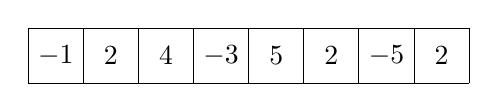
\begin{tikzpicture}[scale=0.7]
\draw (0,0) grid (8,1);

\node at (0.5,0.5) {$-1$};
\node at (1.5,0.5) {$2$};
\node at (2.5,0.5) {$4$};
\node at (3.5,0.5) {$-3$};
\node at (4.5,0.5) {$5$};
\node at (5.5,0.5) {$2$};
\node at (6.5,0.5) {$-5$};
\node at (7.5,0.5) {$2$};
\end{tikzpicture}
\end{center}
\begin{samepage}
el siguiente subarreglo produce la suma máxima $10$:
\begin{center}
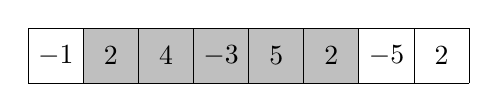
\begin{tikzpicture}[scale=0.7]
\fill[color=lightgray] (1,0) rectangle (6,1);
\draw (0,0) grid (8,1);

\node at (0.5,0.5) {$-1$};
\node at (1.5,0.5) {$2$};
\node at (2.5,0.5) {$4$};
\node at (3.5,0.5) {$-3$};
\node at (4.5,0.5) {$5$};
\node at (5.5,0.5) {$2$};
\node at (6.5,0.5) {$-5$};
\node at (7.5,0.5) {$2$};
\end{tikzpicture}
\end{center}
\end{samepage}

Suponemos que se permite un subarreglo vacío,
por lo que la suma máxima del subarreglo es siempre al menos $0$.
\subsubsection{Algoritmo 1}

Una forma sencilla de resolver el problema
es recorrer todos los subarreglos posibles,
calcular la suma de valores en cada subarreglo y mantener
la suma máxima.
El siguiente código implementa este algoritmo:

\begin{lstlisting}
int best = 0;
for (int a = 0; a < n; a++) {
    for (int b = a; b < n; b++) {
        int sum = 0;
        for (int k = a; k <= b; k++) {
            sum += array[k];
        }
        best = max(best, sum);
    }
}
cout << best << "\n";
\end{lstlisting}

Las variables \texttt{a} y \texttt{b} establecen el primer y
último índice del subarreglo,
y la suma de valores se calcula en la variable \texttt{sum}.
La variable \texttt{best} contiene la suma máxima encontrada durante la búsqueda.

La complejidad temporal de este algoritmo es $O(n^3)$,
porque contiene tres ciclos anidados 
que recorren la entrada.

\subsubsection{Algoritmo 2}

Es fácil hacer que el algoritmo 1 sea más eficiente
quitando un ciclo de él.
Esto es posible calculando la suma en el mismo
momento en el que se mueve el extremo derecho del subarreglo.
El resultado es el siguiente código:

\begin{lstlisting}
int best = 0;
for (int a = 0; a < n; a++) {
    int sum = 0;
    for (int b = a; b < n; b++) {
        sum += array[b];
        best = max(best, sum);
    }
}
cout << best << "\n";
\end{lstlisting}
Después de este cambio, la complejidad temporal es $O(n^2)$.

\subsubsection{Algoritmo 3}

Sorprendentemente, es posible resolver el problema
en tiempo $O(n)$ \footnote{En \cite{ben86}, este algoritmo lineal
es atribuído a J. B. Kadane, y el algoritmo es a veces
llamado \index{algoritmo de Kadane} \key{algoritmo de Kadane}.}, lo cual significa
que solamente con un ciclo es suficiente.
La idea es calcular, para cada posición del arreglo,
la suma máxima de un subarreglo que termina en esa posición.
Después de esto, la respuesta al problema es la
máximo de esas sumas.

Considere el subproblema de encontrar el subarreglo de suma máxima
que termina en la posición $k$.
Hay dos posibilidades:
\begin{enumerate}
\item El subarreglo solo contiene el elemento en la posición $k$.
\item El subarreglo consta de un subarreglo que termina
en la posición $k-1$, seguido del elemento en la posición $k$.
\end{enumerate}

En este último caso, ya que queremos
encontrar un subarreglo con suma máxima,
el subarreglo que termina en la posición $k-1$
también debe tener la suma máxima.
Por lo tanto, podemos resolver el problema de manera eficiente
calculando la suma máxima del subarreglo
para cada posición final de izquierda a derecha.

El siguiente código implementa el algoritmo:
\begin{lstlisting}
int best = 0, sum = 0;
for (int k = 0; k < n; k++) {
    sum = max(array[k], sum + array[k]);
    best = max(best, sum);
}
cout << best << "\n";
\end{lstlisting}

El algoritmo solamente contiene un ciclo
que recorre la entrada,
por lo que la complejidad temporal es $O(n)$.
Esta también es la mejor complejidad temporal posible,
porque cualquier algoritmo para el problema
tiene que examinar todos los elementos del arreglo al menos una vez.

\subsubsection{Comparación de eficiencia}

Es interesante estudiar cuán eficiente
son los algoritmos en la práctica.
La siguiente tabla muestra los tiempos de ejecución
de los algoritmos anteriores para diferentes
valores de $n$ en una computadora moderna.

En cada prueba, la entrada se generó de forma aleatoria.
El tiempo necesario para leer la entrada no fue
medido.

\begin{center}
\begin{tabular}{rrrr}
arreglo de tamaño $n$ & Algoritmo 1 & Algoritmo 2 & Algoritmo 3 \\
\hline
$10^2$ & $0.0$ s & $0.0$ s & $0.0$ s \\
$10^3$ & $0.1$ s & $0.0$ s & $0.0$ s \\
$10^4$ & > $10.0$ s & $0.1$ s & $0.0$ s \\
$10^5$ & > $10.0$ s & $5.3$ s & $0.0$ s \\
$10^6$ & > $10.0$ s & > $10.0$ s & $0.0$ s \\
$10^7$ & > $10.0$ s & > $10.0$ s & $0.0$ s \\
\end{tabular}
\end{center}

La comparación muestra que todos los algoritmos
son eficientes cuando el tamaño de entrada es pequeño,
pero las entradas más grandes resaltan
diferencias en los tiempos de ejecución.
El algoritmo 1 se vuelve lento
cuando $n=10^4$, y el algoritmo 2
se vuelve lento cuando $n=10^5$.
Solamente el algoritmo 3 puede procesar casi instantáneamente
incluso las entradas más grandes.